%\documentclass[spanish,12pt,a4paper,titlepage,twoside,openright]{scrbook}
\documentclass[12pt,a4paper,titlepage]{report}
%\usepackage[latin1]{inputenc}
\usepackage[utf8]{inputenc}
\usepackage{graphicx}
\usepackage{subfig}
\usepackage{float}
\usepackage{wrapfig}
\usepackage{multirow}
\usepackage{caption}
\usepackage[spanish]{babel}
\usepackage[dvips]{hyperref}
\usepackage{amssymb}
\usepackage{listings}
\usepackage{epsfig}
\usepackage{amsmath}
\usepackage{array}
\usepackage[table]{xcolor}
\usepackage{multirow}
\usepackage{hhline}
\usepackage{cancel}

\usepackage[Sonny]{fncychap}
%\usepackage[Glenn]{fncychap}
%\usepackage[Conny]{fncychap}
%\usepackage[Rejne]{fncychap}
%\usepackage[Bjarne]{fncychap}

\usepackage{subfiles}
\usepackage{framed}
\usepackage{appendix}
\setlength{\topmargin}{-1.5cm}
\setlength{\textheight}{25cm}
\setlength{\oddsidemargin}{0.3cm} 
\setlength{\textwidth}{15cm}
\setlength{\columnsep}{0cm}
%\setkomafont{disposition}{\normalfont\bfseries}
\captionsetup{tablename=Tabla}

\ChNameVar{\bfseries\LARGE\sf}\ChNumVar{\fontsize{62}{65}\selectfont}
\ChTitleVar{\bfseries\LARGE\sf} \ChRuleWidth{2pt} \ChNameAsIs
\ChTitleAsIs
\renewcommand\FmN[4]{}
\newcommand{\HRule}{\rule{\linewidth}{0.5mm}}

\begin{document}


\begin{titlepage}
\begin{center}
\vfill
%\vspace{50cm}
\textsc{\LARGE Facultad de Ingenier\'ia de la Universidad de la Rep\'ublica}\\[1.5cm]
\vspace{2cm}
\textsc{\LARGE Procesamiento Digital de Señales de Audio\\[1cm]Curso 2012}\\[0.5cm]
\vspace{2.3cm}
% Title
\HRule \\[0.4cm]
{ \huge \bfseries Beat Tracking}\\[0.4cm]
\HRule \\[1.5cm]
\vspace{2cm}
% Author and supervisor
%\begin{center}
\begin{minipage}{0.4\textwidth}
\begin{flushleft} \large
\emph{Autores:}\\
%\begin{center}
%\begin{LARGE}
Gonzalo \textsc{Gutiérrez}\\ Mat\'ias \textsc{Tailani\'an}
%\end{LARGE}
%\end{center}
\end{flushleft}
\end{minipage}
%\end{center}
\begin{minipage}{0.4\textwidth}
\begin{flushright} \large
\end{flushright}
\end{minipage}

\vspace{2cm}

\vfill
\begin{figure} [h!]
\centering
\subfloat{
\includegraphics[width=0.25\textwidth]{./pics/logoIIE_transparente.png}}\hspace{1cm}
\subfloat{
\includegraphics[width=0.15\textwidth]{./pics/logo_fing_transparente.png}}\hspace{1cm}
\subfloat{
\includegraphics[width=0.15\textwidth]{./pics/logo_udelar.png}}
\end{figure}

% Bottom of the page
{\large \today}
\end{center}
\end{titlepage}



\chapter*{Introducción}

\vspace*{-1cm}

Al escuchar música una reacción inconsciente muy común es mover el pie golpeando el piso a tiempo con el \textbf{beat}. La tarea computacional que intenta replicar ese comportamiento es conocida como \textbf{beat tracking}.\\

La métrica de la señal se puede pensar como una estructura de pulsos percibidos a diferentes escalas temporales en una pieza musical. Se consideran 3 niveles métricos básicos: el \emph{tatum}, el \emph{tactus} o \emph{beat} y el \emph{compás}. El tatum es el valor en tiempo más pequeño que puede encontrarse en una pieza musical, es la unidad atómica de la pieza. En general los otros valores de duración presentes en la pieza son múltiplos de tatum. El tactus o beat está más relacionado con el aspecto semántico, y está directamente vinculado con el \textbf{tempo} de la pieza. Por último el compás está vinculado con la tasa de cambios armónicos o la duración de un patrón rítmico.\\

El problema del seguimiento de beat o \emph{beat tracking} es un problema todavía abierto, donde se sigue intentando con gran actividad lograr mejorar los resultados del estado del arte. Tiene un atractivo muy importante en sí mismo pensando en aplicaciones como el acompañamiento automático, asistencia a la hora del editado, estudios musicológicos, efectos de música adaptativos, o seguimiento del ritmo de una batería tocando en vivo, pero además es una parte imprescindible de algunos sistemas más complejos para aplicaciones como etiquetado de música, reconocimiento automático del género, análisis de similitud de música y para lograr la \emph{transcripción automática de música}.\\

El presente trabajo presenta un algoritmo de seguimiento de \emph{beat} de una pieza musical y se basa en el trabajo de ``Jo\~ao Lobato Oliveira, Fabien Gouyon, Luis Gustavo Martins, Luis Paulo Reis'', titulado ``IBT: A real time tempo and beat tracking system, presentado en la \emph{$11^a$ International Society for Music Information Retrieval Conference, ISMIR}, en 2010'' (\cite{bib:el_posta}). Dicho trabaja se basa a su vez en el sistema \textbf{BeatRoot}, presentado en (\cite{bib:dixon}): Dixon S., ``Automatic extraction of tempo and beat from expressive performances.'', \emph{Journal of New Music Research}, 2001. De \cite{bib:dixon} se toma la idea de varios \textbf{agentes} compitiendo y llevando varias hipótesis de tempo y fase paralelamente, se agrega robustez ante entradas ruidosas y se implementa en tiempo real. Aún realizando todas las operaciones de forma causal y en tiempo real, se logra obtener resultados comparables con el estado del arte y se convierte además en el primer software \emph{open source} de seguimiento de beat en tiempo real.


\chapter*{Algoritmo}

Como se puede ver en la figura \ref{fig:bloques} el algoritmo consta de 3 fases fundamentales:
\begin{itemize}
\item \textbf{Audio Feature Extraction}: En esta etapa se trasforma la señal de audio en 1 secuencia contínua que caracteriza la información más relevante para el análisis rítmico. En esta etapa se basarán las siguientes partes del algoritmo.
\item \textbf{Pre-Tracking}: Al finalizar el Pre-Tracking se tendrá un conjunto de hipótesis iniciales con respecto a posibles períodos y fases de los beats. Consta de 3 subetapas donde se estimarán las características que definen a un agente:
\begin{itemize}
\item Período
\item Fase
\item Puntaje
\end{itemize}
\item \textbf{Beat-tracking}: En esta etapa se propagan las hipótesis y se crean, matan y puntúan agentes.
\end{itemize}

A su vez se presenta un sistema de evaluación que decide en función del puntaje de cada agente, cúal es el más adecuado para la pieza musical: el \textbf{Agent Referee}.

\begin{figure}[h!]
\centering
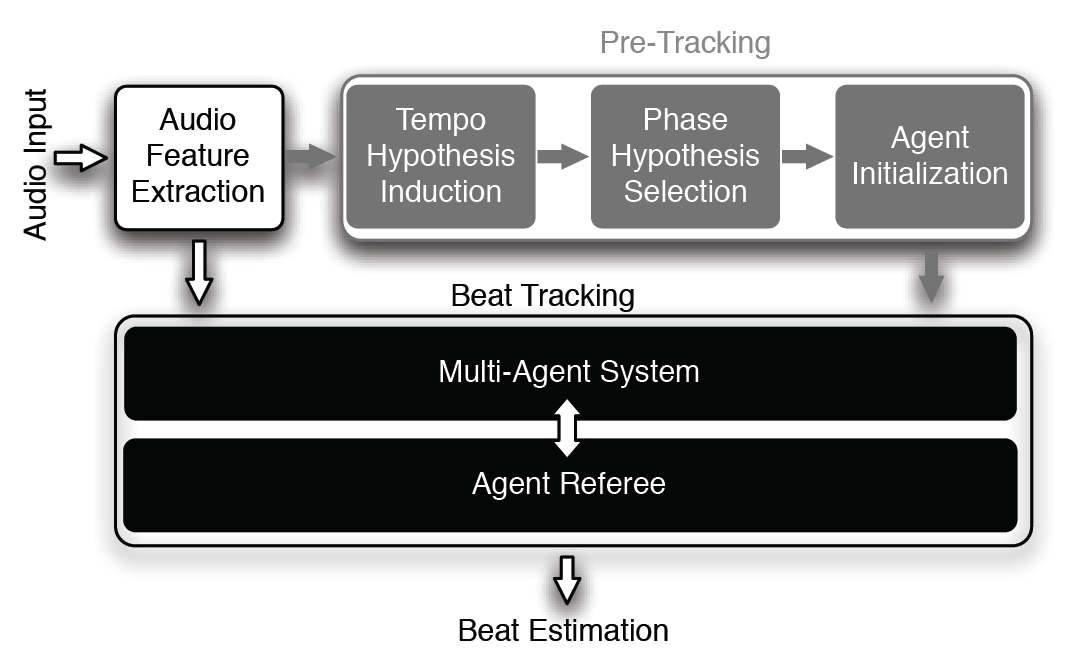
\includegraphics[width=.6\linewidth]{./pics/bloques}
\caption{Diagrama de bloques}
\label{fig:bloques}
\end{figure}

\section*{Audio Feature Extraction}

\section*{Pre-Tracking}

\vspace*{15pt}
	\begin{itemize} \item \textbf{Período} \end{itemize}
	\begin{equation*}
		A(\tau) = \sum\limits_{n=0}^{m}SF(n)SF(n+\tau)
		\label{ec:autocorrelacion}
	\end{equation*}
	$SF$ es el flujo espectral suavizado para el \emph{frame} $n$
	\begin{equation*}
		\begin{cases}
		P_i = \arg\max_i \left\{ A(\tau) \right\}, & i=1,\dots, N\\
		A(\tau)>\delta \frac{rms(A(\tau))}{M} & 
		\end{cases}
		\label{ec:period}
	\end{equation*}
$\delta$ es un umbral determinado empíricamente y $M$ es un rango de tiempos definido entre [50,250] BPM.

\begin{itemize} \item \textbf{Fase} \end{itemize}
Para cada $P_i$ estimado se generan varias hipótesis para la fase: $\phi_i^j$. Se supone fase y períodos constantes en cada ventana de análisis.\\

Se utiliza un \emph{template} de tren de pulsos para ver cuál ajusta mejor.\\[.5cm]
\begin{itemize} \item \textbf{Agentes} \end{itemize}
Para cada pareja $(P_i,\phi_i)$ se computa la suma de errores entre el template de tren de pulsos y los máximos del flujo espectral



\section*{Beat-Tracking}

Idea\\
Supervisar flujo de entrada y mantener balance entre inercia y rapidez de la respuesta\\

Niveles de toleracia: $T_{in}\in[T_{in}^l,T_{in}^r]$ y $T_{out}\in[T_{out}^l,T_{in}^l] \bigcup [T_{in}^r,T_{out}^r]$

\begin{figure}[h!]
  \begin{center}
  \vspace*{-10pt}
  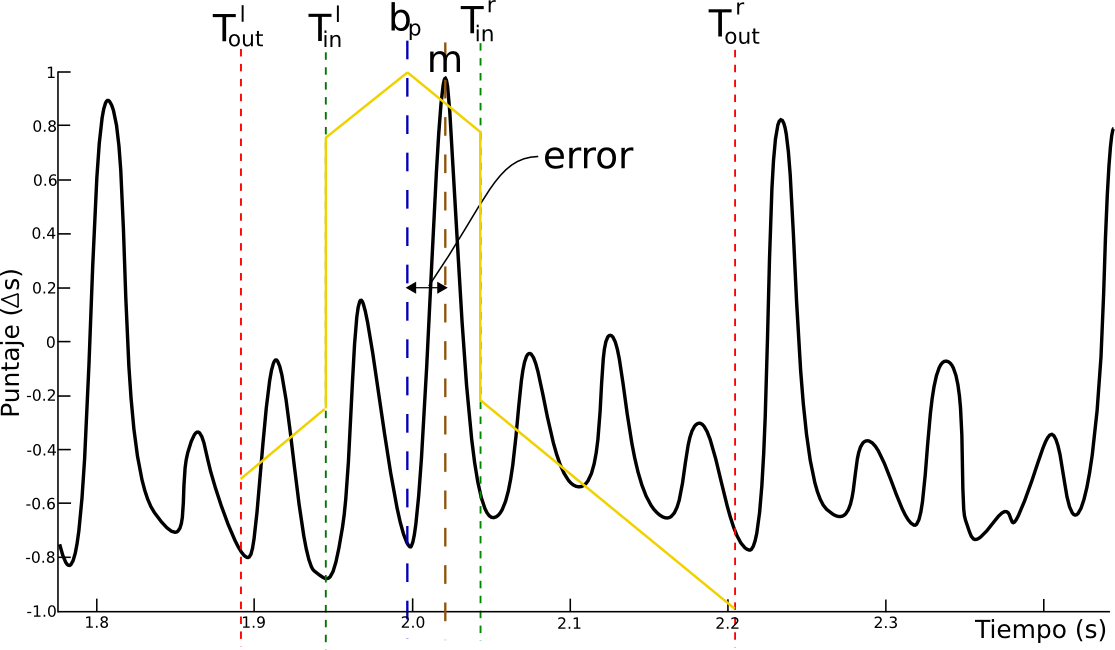
\includegraphics[width=.8\textwidth]{./pics/graficamejor.png}
  \end{center}
  \vspace{-10pt}
  \caption{Niveles de tolerancia}
  \label{fig:grafica}
\end{figure}

\begin{itemize} \item \textbf{$T_{in}\in[T_{in}^l,T_{in}^r]$} \end{itemize}
$$
\begin{cases}
P_i = P_i+0.25*error\\
\phi_i = \phi_i+0.25*error
\end{cases}
$$
\begin{itemize} \item \textbf{$T_{out}\in[T_{out}^l,T_{in}^l] \bigcup [T_{in}^r,T_{out}^r]$} \end{itemize}
El agente mantiene su período y fase y además crea 3 ``hijos'' variando dichos parámetros\\

Agent REferee\\
Evalúa la distancia entre la predicción del \emph{beat} ($b_p$) y el máximo local ($m$) de $SF$. $P_m$ es el máximo período permitido\\
$$\begin{cases}
\Delta s = \left(1-\frac{|error|}{T^r_{out}} \right)\frac{P_i}{P_m}SF(m), & \exists m \in T_{in}\\
\Delta s = -\left(\frac{|error|}{T^r_{out}} \right)\frac{P_i}{P_m}SF(m), & \exists m \in T_{out}\\
\end{cases}$$



\section*{Referencias}
\begin{thebibliography}{99}
\begin{small}

\bibitem{bib:el_posta}Jo\~ao Lobato Oliveira, Fabien Gouyon, Luis Gustavo Martins, Luis Paulo Reis, IBT: A real time tempo and beat tracking system, In \emph{11th International Society for Music Information Retrieval Conference, ISMIR}, 2010.

\bibitem{bib:dixon}S. Dixon. Automatic extraction of tempo and beat from
expressive performances. In \emph{Journal of New Music Research, 30(1):39–58}, 2001.

\bibitem{bib:otra_cosa}S. Dixon. Onset detection revisited. In \emph{in Proceedings of the 9th International Conference on Digital Audio Effects}, pages 133–13, Montreal, Canada, 2006.

\bibitem{bib:y_asi}F. Gouyon, P. Herrera, and P. Cano. Pulse-dependent analyses of percussive music. In \emph{AES 22nd International Conference on Virtual}, Synthetic and Entertainment Audio, 2002.

\end{small}
\end{thebibliography}

\end{document}